\documentclass[12pt,a4letter]{article}
\usepackage{amsmath,amsxtra,amssymb,latexsym, amscd,amsthm}
\usepackage{indentfirst}
\usepackage[mathscr]{eucal}
\usepackage{graphicx}
%\usepackage{txfonts}
\usepackage{picinpar}
\usepackage{floatflt}
\usepackage[utf8]{vietnam}
\usepackage{epic}
\usepackage{makeidx}
\usepackage{longtable}%
\usepackage{multicol}%
%\voffset=-0.8in
% \hoffset=-2cm
\voffset=-2cm
\textheight 24truecm 
\textwidth 16truecm 
\setlength{\baselineskip}{16truept}
\usepackage{answers}
\newtheorem{btbt}{Câu}%[btdb][nosolutionfiles]
\newenvironment{cauhoi}{\begin{btbt}\rm }{\end{btbt}}
\Newassociation{traloi}{Soln}{goiytraloi}
\renewcommand{\Solnlabel}[1]{{\bf Lời giải #1}.}
\def\tentruong{\small ĐH KHOA HỌC TỰ NHIÊN HÀ NỘI}
\def\tenkhoa{Khoa Toán - Cơ -Tin học}
\def\loaidethi{\textbf{Đề số 2}}%{ĐỀ THI LẠI}%%{ĐỀ CHÍNH THỨC}
\def\tenkythi{ĐỀ THI HỌC KÌ 2017-2018}
\def\tenmonhoc{Môn thi: Lý thuyết tối ưu}
\def\thoigian{Thời gian làm bài: 90 phút}
\usepackage{centerpage}
\usepackage{mathpazo}
\usepackage{systeme}
\sysdelim.. \syseqsep{:}
\graphicspath{{hinh/}}
\begin{document}
\Opensolutionfile{goiytraloi}[traloi] 
\Writetofile{goiytraloi}{\protect\centerline{\bf LỜI GIẢI: \tenkythi - SỐ 2}}
\thispagestyle{empty}
\begin{minipage}[b]{0.45\textwidth}
\centering
{ \tentruong}\\
\tenkhoa\\ %\makebox[4cm]{\hrulefill}\\
\loaidethi\\
\quad \\
%{({\it Đề thi \@scau{} câu / \@strang{} trang})}
\end{minipage}
\hfill
\begin{minipage}[b]{0.5\textwidth}
\centering
{\bf \tenkythi}\\
{\bf  \tenmonhoc}\\
{\it \thoigian}\\
\qquad %{\it \@scau}
\end{minipage}


\vspace*{1cm}

\begin{cauhoi}%1
(3 điểm) 
Tìm các phương án cực biên không suy biến của bài toán
$$f(x)=2x_1-x_2+3x_3\rightarrow\max$$
$$\begin{cases}
\systeme{
x_1 +x_2  +  x_3+x_4  =  10,:
2x_2  +x_3 -x_4 =  6,}\\
x_j \ge 0, j = 1, 2, 3,4.
\end{cases}$$

%%%%%%%%%%%%%%%%%lời giải
\begin{traloi}
Bài toán này có $m = 2$ ràng buộc chính và $n = 4$ biến. Một phương án cực biên có nhiều nhất $m = 2$ thành phần dương, tức là có ít nhất $n - m = 2$ thành phần $= 0$.
Vì thế, lần lượt cho mỗi cặp biến$ x_1, x_2, x_3, x_4 = 0$ ta được:\\
Với $x_1 = x_2 = 0$, hệ phương trình trên cho ta $x_3 = 8; x_4 = 2$.\\
Với $x_1 = x_3 = 0$, hệ phương trình  cho ta $x_2 = \dfrac{16}{3}; x_4 = \dfrac{14}{3}$.\\
Với $x_1 = x_4 = 0$, hệ phương trình  không có nghiệm không âm.\\
Với $x_2 = x_3 = 0$, hệ phương trình  không có nghiệm không âm.\\
Với $x_2 = x_4 = 0$, hệ phương trình  cho ta $x_1 = 4; x_3 = 6$.\\
Với $x_3 = x_4 = 0$, hệ phương trình  cho ta $x_1 = 7; x_2 = 3$.

Như vậy ta nhận được các phương án sau đây:
$$x_1 = (0, 0, 8, 2)^T;   x_2 = \left(0, \dfrac{16}{3}, 0, \dfrac{14}{3}\right)^T; $$
$$  x_3 = (4, 0, 6, 0)^T;   x_4 = (7, 3, 0, 0)^T.$$

Kiểm tra trực tiếp cho thấy cả 4 phương án trên đều là các phương án cực biên không suy biến (do số thành phần dương $m=2$).
\end{traloi}
\end{cauhoi}

\begin{cauhoi}%2
(3 điểm)  
Giải bài toán quy hoạch tuyến tính sau bằng phương pháp hình học
\begin{center}
$ f(x,y)=2x+y\rightarrow\min $\\
 $\begin{cases}
\systeme{
2x+y\ge 2,:
-x+2y\le 6,: 
5x-y\le 15,}\\ 
x,y\ge 0.
\end{cases} $
\end{center}
\begin{traloi}
Giải bằng phương pháp hình học. 
Miền xác định các phương án trong ngũ giác lồi $ABCDE$ với $A(0,2), B(0,3), C(4,5), D(3,0), E(1,0)$. Vectơ pháp tuyến của đường thẳng hàm mục tiêu $L(x,y)=2x+y$ là $\vec{n}=(2,1)$.

\begin{figure}[!ht]
\centering
% \input hinh13.tex
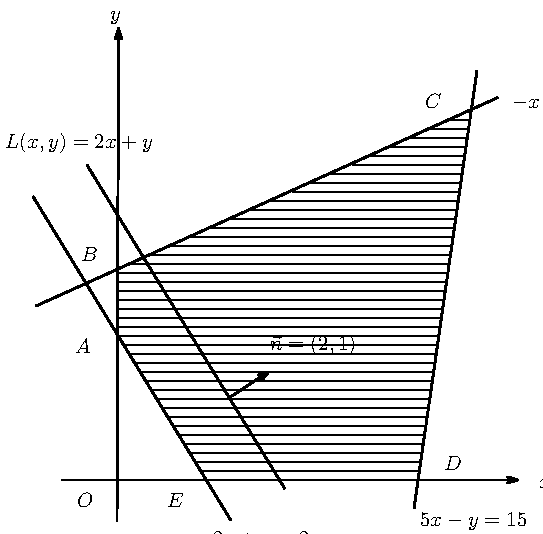
\includegraphics[scale =0.7]{hinh13}
\caption{}\label{fig:h1}
\end{figure}

Do hàm mục tiêu đòi hỏi $\min$, di chuyển hàm mục tiêu ngược chiều với vectơ pháp tuyến  . Bài toán có  nghiệm là đoạn $[A,E]$.  
\end{traloi}
\end{cauhoi}

\begin{cauhoi}%2
(4 điểm)  
Cho bài toán quy hoạch tuyến tính
\begin{center}
 $ f(x)=5x_1+4x_2+5x_3+2x_4+x_5+3x_6\rightarrow\min $\\
$ \begin{cases}
\systeme{
2x_1+4x_2+3x_3+x_4= 52,:
4x_1+2x_2+3x_3+x_5=60,:
3x_1+x_3+x_6=36,}\\
x_i\ge 0, i=1,2,3,4,5,6.
\end{cases} $
\end{center}

Giải bài toán theo phương pháp đơn hình.

%%%%%%%%%%%%%%%%%lời giải
\begin{traloi}
1. Dễ thấy có cơ sở $J={4,5,6}$ với $x^0=(0,0,0,52,60,36)^T$ là một phương án cực biên của bài toán đã cho, từ đây ta có bảng đong hình

\begin{center}
\renewcommand{\arraystretch}{1.25}
\begin{tabular}{| l | l | l | l | l | l | l | l | l | l|}
\hline
$J$&$c_J$&$x_J$&1&2&3&4&5&6\\ 
\cline{4-9}
&&&5&4&5&2&1&3\\ 
\hline
4&2   &52   &2  &4 &3 &1&0&0\\
5&1   &60    &4 &2&3 &0&1&0\\
6&3   &36    &\textbf{(3)} &0&1&0&0&1\\
\hline
&&272&\textbf{[12]}&6&7& 0&0&0\\
\hline
4&2   &28   &0  &4 &$\frac{7}{3}$&$1$&0&$-\frac{2}{3}$\\
5&1  &12    &0   &\textbf{(2)}&$\frac{5}{3}$ &0&1&$-\frac{4}{3}$\\
1&5   &12    &1  &0&$\frac{1}{3}$ &0&0&$\frac{1}{3}$\\
\hline
&&128 &0&\textbf{[6]}& 3& 0&0&-4\\
\hline
4&2   &4   &0  &0 &-1&1&-2&2\\
2&4  &6    &0   &1&$\frac{5}{6}$ &0&$\frac{1}{2}$&$-\frac{2}{3}$\\
1&5   &12    &1&0&$\frac{1}{3}$ &0&0&$\frac{1}{3}$\\
\hline
&&92 &0&0& -2& 0&-3&0\\
\hline
\end{tabular}
\end{center}
Phương án tối ưu là $x^*=(12,6,0,4,0,0)$, $L(x^*)=92.$
\end{traloi}
\end{cauhoi}

%%%%%%%%%%%%%%%%%%%%
\Closesolutionfile{goiytraloi}
\newpage
\Readsolutionfile{goiytraloi}

\end{document}